\documentclass[border=4pt]{standalone}

% --- packages (mirror these in matrix.meta.json "requires") ---
\usepackage{tikz}
\usetikzlibrary{decorations.pathreplacing}

% --- palette (canonical source: reference/color-palettes/color-palettes.md; light variant) ---
\definecolor{otblue}{HTML}{0072B2}
\definecolor{otorange}{HTML}{E69F00}
\definecolor{otteal}{HTML}{009E73}
\definecolor{otpurple}{HTML}{CC79A7}
\definecolor{otgray}{HTML}{5A5A5A}

\begin{document}
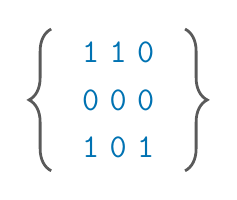
\begin{tikzpicture}
  % enclosing curly braces (neutral structure color)
  \draw[otgray, line width=1pt, decorate, decoration={brace, amplitude=8pt}]
    (-0.3,-0.05) -- (-0.3,1.75);
  \draw[otgray, line width=1pt, decorate, decoration={brace, amplitude=8pt, mirror}]
    (1.4,-0.05) -- (1.4,1.75);
  % binary matrix of bits (data-coloured)
  \begin{scope}[every node/.style={font=\ttfamily\large\bfseries, text=otblue}]
    % row 1: 1 1 0
    \node at (0.2,1.45) {1}; \node at (0.55,1.45) {1}; \node at (0.9,1.45) {0};
    % row 2: 0 0 0
    \node at (0.2,0.85) {0}; \node at (0.55,0.85) {0}; \node at (0.9,0.85) {0};
    % row 3: 1 0 1
    \node at (0.2,0.25) {1}; \node at (0.55,0.25) {0}; \node at (0.9,0.25) {1};
  \end{scope}
\end{tikzpicture}
\end{document}
